\subsection{Performance Portability Visualization}
\label{sec:pp_visualization}

Since the tables presented in the previous section can get quite large and difficult to understand, it is advisable to use some form of visualization to help readers grasp the most important results, especially characteristics, as easily and quickly as possible. 

To visualize the performance efficiencies shown in \autoref{tab:example_effs}, the most widely used solution in the literature is to use a heatmap as depicted in \autoref{fig:vis_example_effs} using the data from \autoref{tab:example_effs}.

\begin{figure}
    \centering
    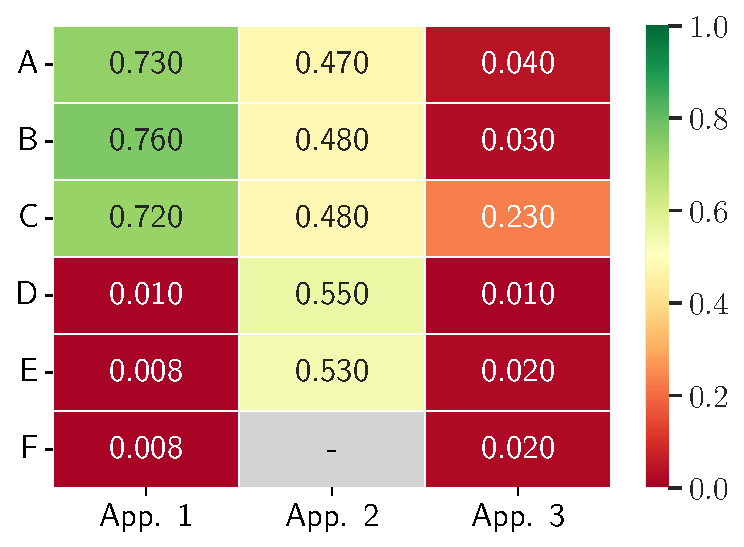
\includegraphics[width=0.75\linewidth]{figures/02_performance_portability/example_diss_eff_heat.pdf}
    \caption{%
    An example visualization of the architectural efficiencies (higher is better) of \autoref{tab:example_effs} as a heatmap. 
    This visualization makes it easy to spot the overall behavior of the three example applications. 
    }
    \label{fig:vis_example_effs}
\end{figure}

Such heatmaps make it easy to see the different application characteristics at a glance, including the cases where an application does not support a hardware platform. 
However, care must be taken to scale the heatmap to the same range, in case of performance efficiencies, the range $\interval{0}{1}$, regardless of the actual values, to make different heatmaps easier comparable. 

However, visualizing the performance portability metrics without losing or obscuring too much information is more difficult. 
In their paper, \citet{sewall_interpreting_2020} compared different visualization techniques for their \pp metric and discussed their advantages and disadvantages. 
They concluded that established visualization techniques like box plots, histograms, probability density functions, or violin plots in theory work, but they all lose or obscure some information, mostly when an application does not support a hardware platform.
They concluded that now-established visualization techniques cannot convey all important information, especially if we factor in the importance of the used platform set in the calculation of \pp. 
Therefore, based on the idea in \cite{deakin_performance_2019}, \citet{sewall_interpreting_2020} proposed the efficiency cascade plots and platform charts. 
Such an example plot for the performance efficiencies in \autoref{tab:example_effs} and performance portability scores of \pp in \autoref{tab:example_perfs} is shown in \autoref{fig:vis_example_pp}.

\begin{figure}
    \centering
    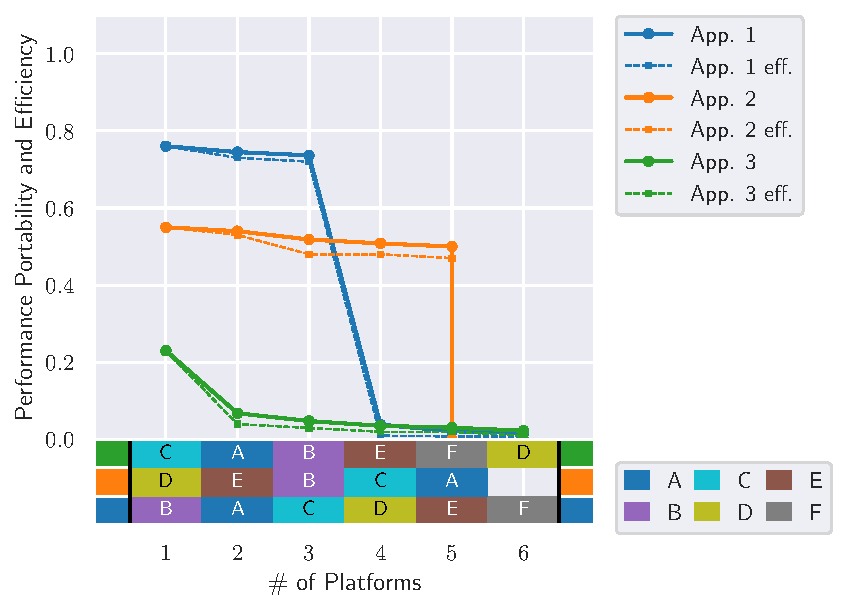
\includegraphics[width=\linewidth]{figures/02_performance_portability/example_diss_eff_cascade.pdf}
    \caption{%
    An example visualization of the architectural efficiencies of \autoref{tab:example_effs} and performance portability scores of \autoref{tab:example_pp} for \pp for the three example applications as proposed by \citet{sewall_interpreting_2020}. 
    This plot can help us to determine the set of platforms best supported by some applications. 
    }
    \label{fig:vis_example_pp}
\end{figure}

Creating an efficiency cascade plot works as follows. 
First, each application's \pp and efficiency values are gathered using all hardware platforms. 
Afterward, the platform with the smallest remaining efficiency is removed and the now-reduced platform set as a new baseline to calculate the next \pp score. 
This process is repeated until only one platform, the best-performing platform for the current application, is left in the platform set. 
These values are then plotted from right to left, resulting in a monotonically decreasing plot of the performance portability scores and efficiencies. 
Alternatively, the new \enquote{P3 explorer} project can be used to automate the creation of a efficiency cascade plot~\cite{smith_p3_2024, smith_p3-explorerp3-explorergithubio_2024}. 

As discussed by \citet{sewall_interpreting_2020, pennycook_navigating_2021}, this plot can be used to draw many different conclusions from the raw \pp and performance efficiency values. 
Applications for which the efficiency cascade plot extends further to the right support more hardware platforms and are, therefore, more portable. 
Also, we can directly see how many platforms are supported and which platforms have the highest performance efficiencies. 
This can help us identify whether our application's performance in one architectural class is lackluster and needs to be addressed. 
One drawback of the efficiency cascade plots is that one must be careful since the order of hardware platforms in the platform charts at the bottom of the plot may differ for each application. 

For an example, we can look at \autoref{fig:vis_example_pp}. 
For application one, we see that the platforms from the first architectural class are supported best, followed by a sharp decline in performance portability after adding platforms from the second class. 
On the other hand, application two's performance portability scores are, on average, better for more hardware platforms until platform F is added, which results in a score of zero, shown by a vertical decline in the plot. 
Application three also shows bad performance portability scores for all hardware platforms, as already discussed. 


The efficiency cascade plots were created only with \pp in mind. 
Creating the same plot for the \mpp metric is not directly possible since, per \autoref{def:mpp}, only platforms with the same architectural class should be used to calculate \mpp. 
However, if we relax this restriction and use all platforms when calculating \mpp, we can also create an efficiency cascade plot for scores retrieved via \mpp. 

\begin{figure}
    \centering
    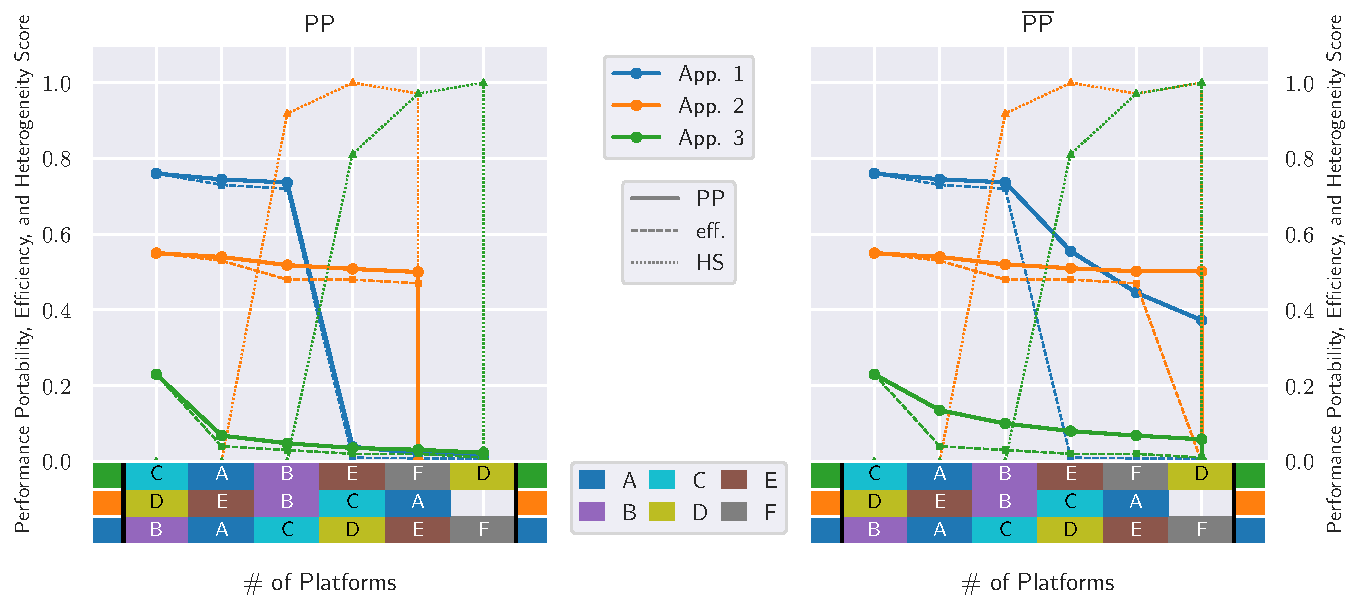
\includegraphics[width=\linewidth]{figures/02_performance_portability/example_diss_eff_cascade_both_HS.pdf}
    \caption{%
    An example visualization of the architectural efficiencies of \autoref{tab:example_effs} and performance portability scores of \autoref{tab:example_pp} for the three example applications as proposed by \citet{sewall_interpreting_2020}. 
    On the left-hand side, the scores for \pp proposed by \citet{pennycook_implications_2019} are plotted, and on the right-hand side, the scores for \mpp proposed by \citet{marowka_comparison_2023}. 
    Additionally, both plots contain the newly proposed heterogeneity score $HS$ (\autoref{def:hetero_score}) as dotted lines. 
    }
    \label{fig:vis_example_both_hs}
\end{figure}

\autoref{fig:vis_example_both_hs} displays the same plot as \autoref{fig:vis_example_pp} but now showing both performance portability metrics, \pp (left-hand side) and \mpp (right-hand side). 
Additionally, the newly proposed heterogeneity score $HS$ is added as dotted lines. 
The plot on the left shows that while application one has a high \pp score, its heterogeneity score is zero in our example, meaning only a single architectural class is highly optimized. 
On the other hand, application two's \pp score is lower, but its heterogeneity score is higher, meaning its \pp score of roughly $\num{0.5}$ is not caused by only one architectural class being optimized but multiple. 
This new heterogeneity score plot nicely complements the efficiency cascade plot and the platform chart, making the results easier and better interpretable. 

Looking at the efficiency cascade plot of the \mpp metric, we can see that due to the usage of the arithmetic mean, the correlation between the \mpp values and the corresponding performance efficiencies is not as high as with the \pp metric. 
